\section{Club-Level Applications}
\label{sec:club_applications}

This section demonstrates the practical application of club-level models to real \textit{Brasileirão} seasons from 2020 to 2025.
Using one of the best-performing models from Section~\ref{sec:real_data} (P7) and the season-level simulation approach described in Section~\ref{sec:evaluation_methodology}, we illustrate how the model generates probabilistic forecasts for championship outcomes.
While Section~\ref{sec:real_data} evaluated all club-level models across multiple seasons using quantitative scoring rules, here we focus on a single well-performing model and examine specific seasons in depth, providing qualitative insights into how probabilistic forecasts evolve and how the model captures the real championship race.
We select specific seasons that showcase different aspects of the model's behaviour: competitive title races, historic relegations, and the inherent uncertainty of football.
Other seasons have their graphics available in the Appendix~\ref{appendix:season_level_simulations}.

\subsection{2020 Season}
\label{subsec:season_2020}

The 2020 season was played under the unique circumstances of the COVID-19 pandemic, with a calendar that started in August 2020 and extended into February 2021.
This season produced one of the most competitive title races in recent memory, with four clubs trading positions as favourites throughout the campaign.

Figure~\ref{fig:2020_champ} shows how Internacional, São Paulo, Atlético Mineiro, and Flamengo alternated as title favourites.
No club maintained a sustained lead: Atlético Mineiro reached approximately 70\% probability in October, while São Paulo and Internacional reached near 80\% in December and January, respectively.
Flamengo, who had remained competitive throughout the season, secured the title in the final rounds.
The volatility of these probability trajectories, with the leading club changing multiple times, reflects the genuine competitive balance among the top teams.

\begin{figure}[htbp]
    \centering
    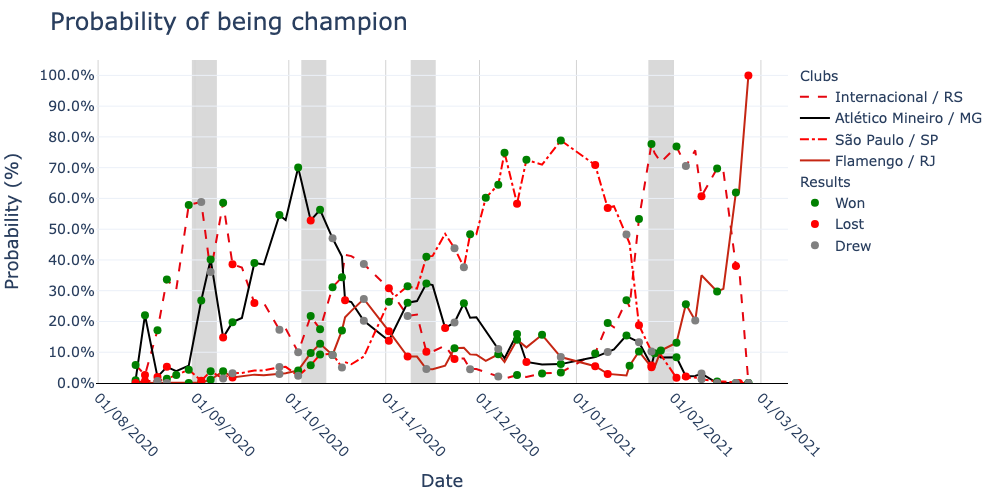
\includegraphics[width=\textwidth]{figures/2020_visualization_poisson_7_champ.png}
    \caption{
        \textbf{Championship probability evolution for the 2020 \textit{Brasileirão}}.
        Each line represents the probability of winning the title for a given club, updated after each match-day.
        Markers indicate individual match results: green circles denote victories, red circles denote defeats, and gray circles denote draws.
        Shaded vertical bands indicate FIFA international periods.
    }
    \label{fig:2020_champ}
\end{figure}

The relegation battle exhibited distinct probability trajectories for different clubs, as shown in Figure~\ref{fig:2020_z4}.
The high probabilities observed in August (Fortaleza over 80\%, Sport and Goiás near 70\%) reflect estimation uncertainty due to limited data: at this stage, each team had played only a few matches, and the posterior estimates are dominated by prior information rather than observed performance.
As more matches were played, the estimates converged to more stable values.
Goiás exhibited a steady increase in relegation probability from October onwards, reaching near-certainty by the final rounds and being mathematically relegated before the last match-day.
Sport maintained high probabilities during the second half of the season.
However, Sport's results improved in the closing stages of the season, while Vasco da Gama's form deteriorated, resulting in Sport avoiding relegation.
On the other hand, Vasco da Gama's trajectory illustrates a progressive deterioration: starting with near-zero probability in August, their estimated relegation risk increased throughout the season, culminating in their relegation.
Fortaleza's probability stabilized at low values once sufficient data accumulated, and they finished comfortably above the relegation zone despite losing their final three matches.

\begin{figure}[htbp]
    \centering
    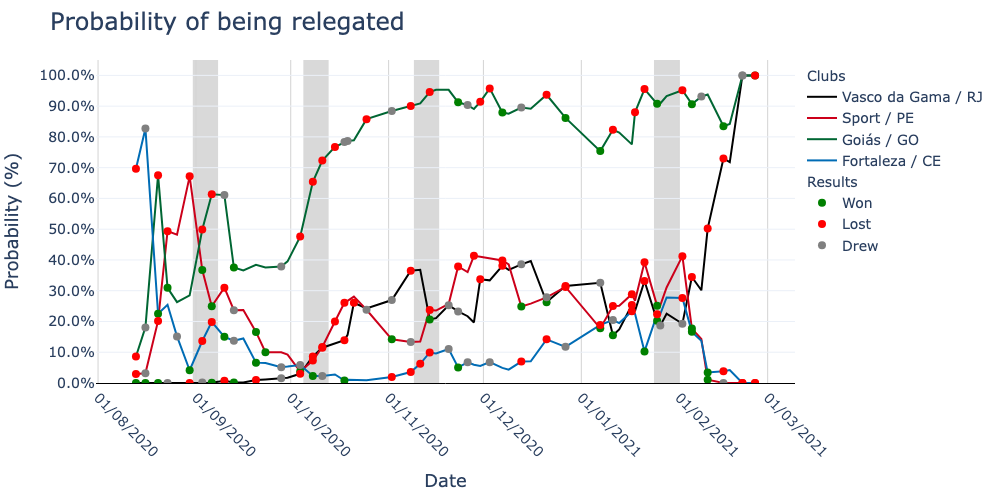
\includegraphics[width=\textwidth]{figures/2020_visualization_poisson_7_z4.png}
    \caption{
        \textbf{Relegation probability evolution for the 2020 \textit{Brasileirão}}.
        Each line represents the probability of relegation (finishing in positions 17--20) for a given club, updated after each match-day.
        Markers indicate individual match results: green circles denote victories, red circles denote defeats, and gray circles denote draws.
        Shaded vertical bands indicate FIFA international break periods.
    }
    \label{fig:2020_z4}
\end{figure}

Figure~\ref{fig:heatmap_2020} shows the mid-season position distribution for all 20 clubs after 192 matches (approximately half the season).
Each cell represents the probability of a club finishing in a given position, with brighter colours indicating higher probabilities.

The heatmap reveals a clear stratification of the league at mid-season.
At the top, São Paulo leads with 31.46\% probability of winning the title, followed by Atlético Mineiro (26.11\%), Internacional (21.78\%), and Flamengo (8.61\%).
São Paulo shows the highest concentration in the top four positions (79.31\%), followed by Atlético Mineiro (78.23\%) and Internacional (74.83\%).
Flamengo, while still a title contender, exhibits a more diffuse distribution with only 52.96\% probability of finishing in the top four, extending into positions 5--7.
Palmeiras shows probability mass concentrated in positions 4--8, with 59.84\% probability of finishing in the top six, indicating a strong campaign at mid-season.

The middle of the table displays considerable uncertainty, though with small identifiable clusters.
Fluminense and Grêmio show their probability mass concentrated in positions 4--8, while Santos exhibits a similar concentration shifted slightly lower to positions 5--9.
Further down, Fortaleza's distribution places its mass of probability in positions 7--11.
These wide intervals, spanning 5 to 7 positions each, reflect the difficulty in distinguishing teams of similar quality based on partial-season data.

At the bottom, the relegation picture shows varying degrees of certainty.
Goiás exhibits highly concentrated probability mass in position 20 and has 90.02\% probability of relegation (positions 17--20).
Botafogo (42.81\% relegation probability), Red Bull Bragantino (40.94\%), Coritiba (41.54\%), and Athlético Paranaense (51.53\%) show distributions concentrated in the lower positions, indicating significant relegation risk.

\begin{figure}[htbp]
    \centering
    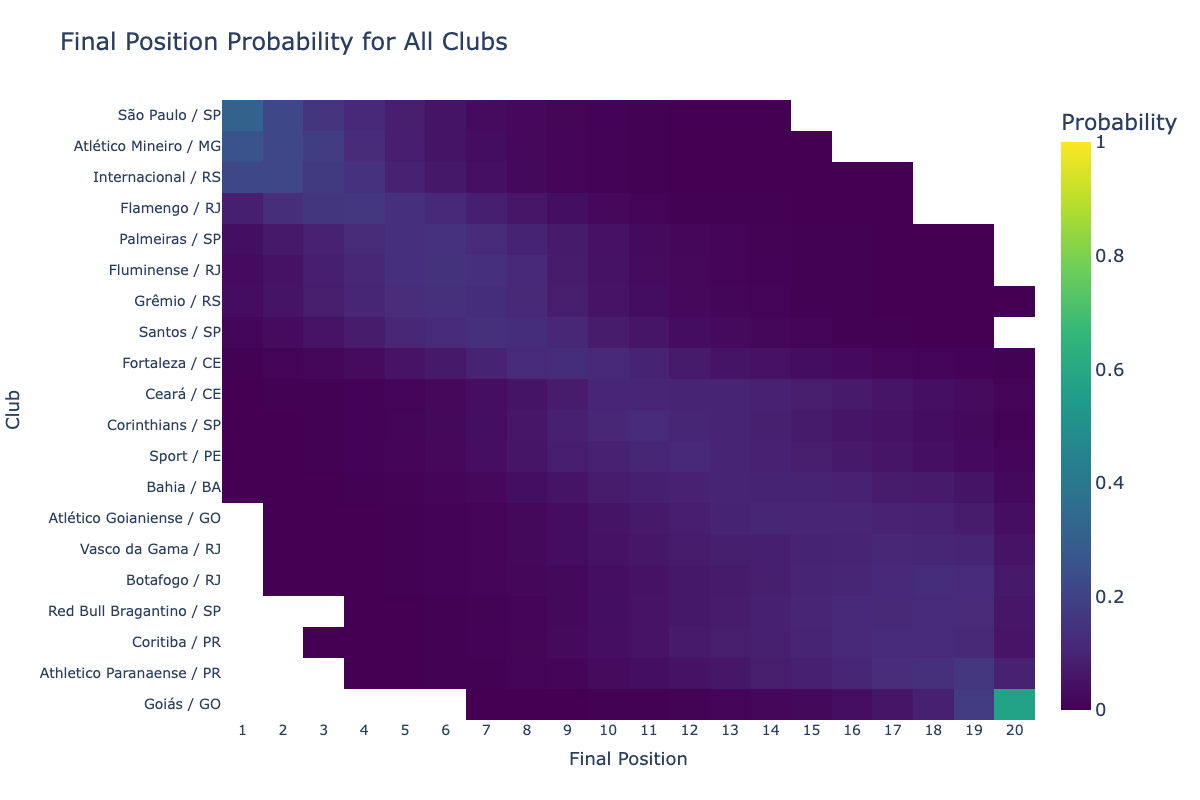
\includegraphics[width=\textwidth]{figures/2020_final_position_probs_all_clubs_192_poisson_7.png}
    \caption{
        \textbf{Final position probability distribution at mid-season 2020 (after 192 matches)}.
        Each cell shows the probability of a club (row) finishing in a given position (column), estimated from 10,000 Monte Carlo simulations.
        Clubs are ordered vertically by expected final position, with brighter colours indicating higher probabilities.
    }
    \label{fig:heatmap_2020}
\end{figure}

The end-of-season team strength estimates are shown in Figure~\ref{fig:team_strengths_2020}.
The violin plots display posterior distributions of the team strength parameter (in log scale) for each club, ordered by estimated median strength.

The figure reveals the competitive nature of this season through the extensive overlap of posterior distributions.
Among the title contenders, Internacional shows the highest median strength, but the median strengths of Flamengo up to Red Bull Bragantino are all very similar, indicating that these clubs possessed similar underlying quality.

In the middle of the table, something similar happens to Ceará, Athlético Paranaense, Santos and Corinthians.
Also, Atlético Goianiense, Fortaleza and Bahia show similar median strengths.
At the bottom, the relegated clubs (Vasco da Gama, Goiás, Coritiba and Botafogo) join Sport to form another group of clubs with similar median strengths.

The distributions of Internacional and Botafogo do not overlap with each other, nor with most other clubs: Internacional's distribution lies entirely above the average (zero), while Botafogo's lies entirely below.
For the remaining clubs, considerable overlap exists among the distributions, particularly within the mid-table group, making it difficult to distinguish teams based on strength estimates alone.

\begin{figure}[htbp]
    \centering
    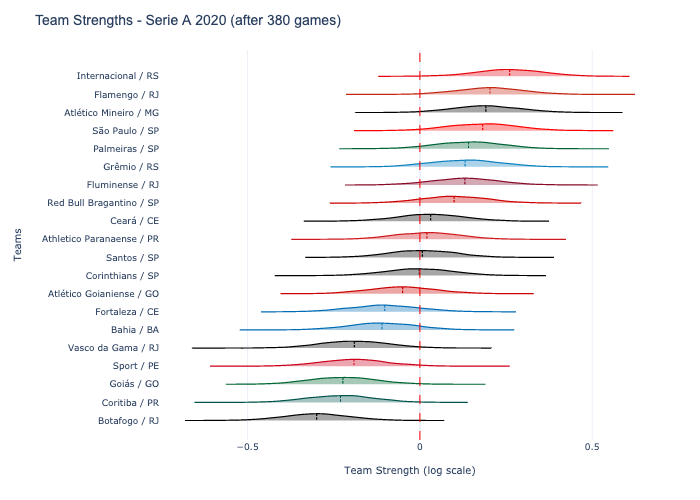
\includegraphics[width=0.9\textwidth]{figures/2020_team_strengths_violin.png}
    \caption{
        \textbf{Posterior distributions of team strengths for the 2020 \textit{Brasileirão} (after 380 matches)}.
        Each violin plot shows the posterior distribution of the team strength parameter (log scale) estimated from 4,000 MCMC samples.
        Teams are ordered vertically by posterior median strength, from lowest (bottom) to highest (top).
        The shape of each violin represents the density of the posterior distribution, and the dashed line inside each violin indicates the mean.
        The dashed red vertical line at zero represents the average team strength.
    }
    \label{fig:team_strengths_2020}
\end{figure}

\subsection{2023 Season}
\label{subsec:season_2023}

While the 2020 season had a competitive title race, the seasons 2021 and 2022 saw two solid campaigns, with titles for Atlético Mineiro and Palmeiras, respectively.
The season of 2023 was on track to be another solid campaign, with the high performance of Botafogo, with a difference of 13 points to the second place after 19 matches.
However, the season produced one of the most significant late-season reversals in Brazilian football history.

Figure~\ref{fig:2023_champ} shows the championship probability evolution, dominated by Botafogo from June through October.
By mid-June, Botafogo had a probability of over 60\% to win the title.
With three consecutive victories, Botafogo's probability rose to 90\% in mid-July.
During August, Botafogo's probability remained above 90\%, exceeding 95\% in some points.
September proved challenging, with three consecutive defeats and a draw, but the probability remained around 80\%.

In October, with two consecutive victories, Botafogo's probability returned to above the 90\%, but from October 21 on, Botafogo stopped winning.
In the season's last 11 matches, Botafogo drew six and lost five, including a sequence of four consecutive defeats.
During this period, the second place team, Palmeiras, was able to close the gap by winning 8 matches, including a 3--4 victory over Botafogo, having trailed 3-0 at half-time.
At the end of the season, Palmeiras was the champion, and Botafogo finished in fifth place.

\begin{figure}[htbp]
    \centering
    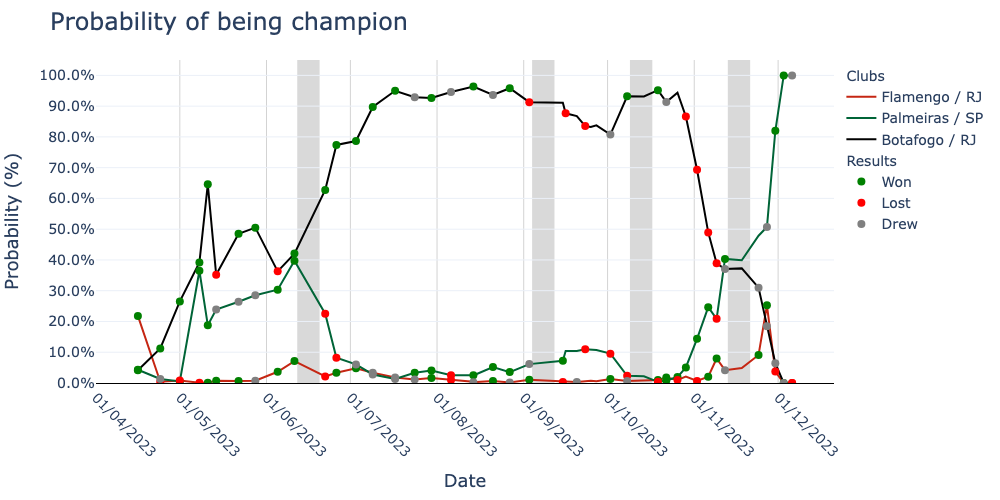
\includegraphics[width=\textwidth]{figures/2023_visualization_poisson_7_champ.png}
    \caption{
        \textbf{Championship probability evolution for the 2023 \textit{Brasileirão}}.
        Each line represents the probability of winning the title for a given club, updated after each match-day.
        Markers indicate individual match results: green circles denote victories, red circles denote defeats, and gray circles denote draws.
        Shaded vertical bands indicate FIFA international break periods.
    }
    \label{fig:2023_champ}
\end{figure}

The relegation battle was equally dramatic, culminating in the first relegation in Santos's 111-year history.
Figure~\ref{fig:2023_z4} shows how the relegation probabilities of Vasco, Bahia, Goiás and Santos oscillated throughout the season.
With a collapse in the title race, the relegation battle also produced an unexpected outcome.
Remaining only one round, América-MG, Coritiba and Goiás were already relegated.
The last club to be relegated was among Bahia, Vasco and Santos.
Bahia were in the relegation zone, with a probability of 59.60\% of being relegated.
Vasco, the first club out of the relegation zone, had a probability of 28.91\%.
Finally, Santos were the favourite to avoid relegation, with a probability of 11.49\%.

On the final round, Santos could avoid relegation by winning their match or, if drawing their match, by Vasco or Bahia not winning their matches.
If Santos lost, they still could avoid relegation if Vasco lost or with Bahia not winning their match.
At the final round, Bahia won the match against Atlético Mineiro, while Vasco won against Red Bull Bragantino.
With a loss to Fortaleza, Santos were relegated.

\begin{figure}[htbp]
    \centering
    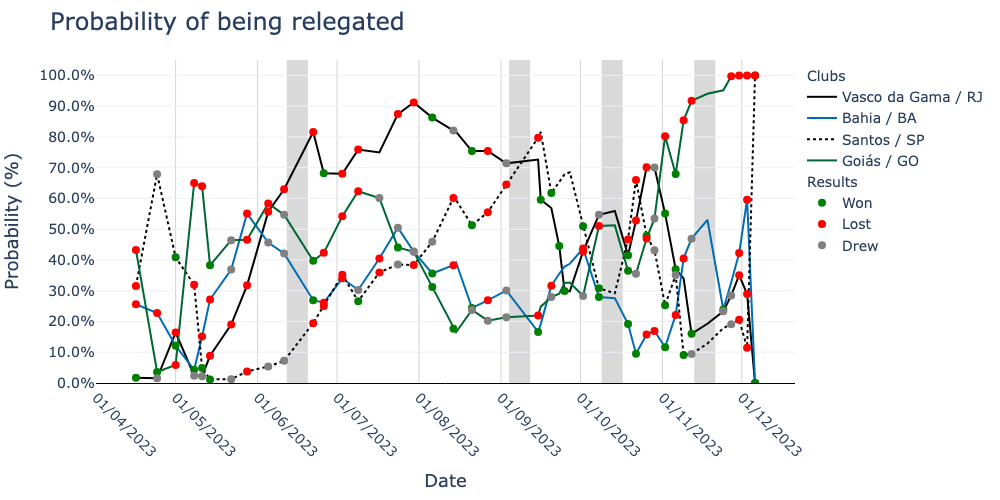
\includegraphics[width=\textwidth]{figures/2023_visualization_poisson_7_z4.png}
    \caption{
        \textbf{Relegation probability evolution for the 2023 \textit{Brasileirão}}.
        Each line represents the probability of relegation (finishing in positions 17--20) for a given club, updated after each match-day.
        Markers indicate individual match results: green circles denote victories, red circles denote defeats, and gray circles denote draws.
        Shaded vertical bands indicate FIFA international break periods.
    }
    \label{fig:2023_z4}
\end{figure}

Figure~\ref{fig:heatmap_2023} shows the mid-season position distribution for all 20 clubs after 188 matches.
The contrast with 2020 is striking: while 2020 exhibited diffuse probabilities at the top reflecting a four-way race for the title, the 2023 heatmap shows extreme concentration, especially on the first and second places.
Botafogo holds 95.98\% probability of winning the title, with the remaining probability distributed between Palmeiras (2.83\%) and negligible amounts for other clubs.
Palmeiras shows probability mass concentrated in positions 2--4, with 79.46\% probability of finishing in the top four.

At the bottom, the relegation picture shows América-MG with near-certain probability of finishing in the relegation zone (96.73\% in positions 17--20).
Coritiba, with 88.17\%, and Vasco, with 81.67\%, also show high relegation probabilities.
Santos exhibits 59.44\% relegation probability at mid-season.
Notably, Bahia shows 39.16\% relegation probability at that point, while Goiás had 16.51\% probability of being relegated.
These values increased at the end of the season due to some losses.

\begin{figure}[htbp]
    \centering
    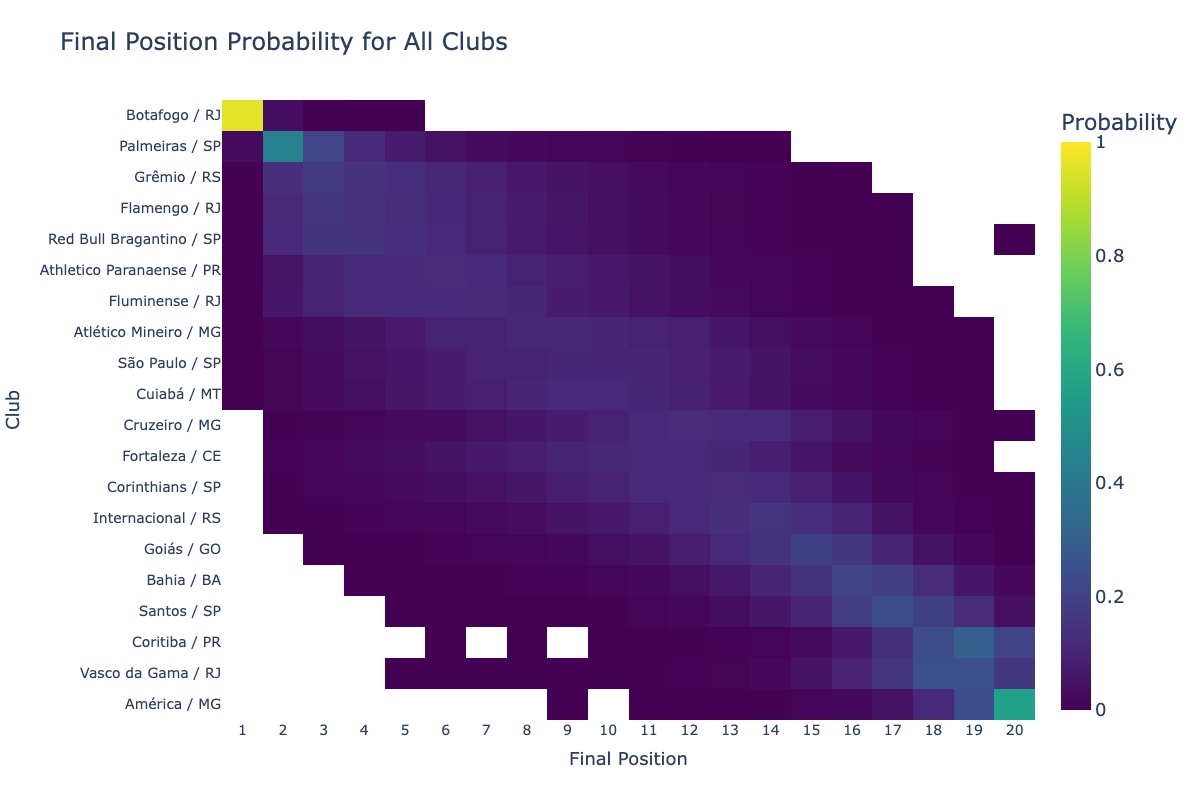
\includegraphics[width=\textwidth]{figures/2023_final_position_probs_all_clubs_188_poisson_7.png}
    \caption{
        \textbf{Final position probability distribution at mid-season 2023 (after 188 matches)}.
        Each cell represents the estimated probability of a club (row) finishing the season in a given position (column), based on 10,000 Monte Carlo simulations of the remaining 192 matches.
        Clubs are ordered vertically by expected final position; brighter colours indicate higher probabilities.
    }
    \label{fig:heatmap_2023}
\end{figure}

The end-of-season team strength estimates are shown in Figure~\ref{fig:team_strengths_2023}.
The violin plots display posterior distributions of the team strength parameter (in log scale) for each club, ordered by posterior median strength.

Like 2020, 2023 does not show a clear separation at the top.
Palmeiras exhibits the highest estimated median strength, followed by Botafogo and Atlético Mineiro, whose distributions show considerable mutual overlap.
Flamengo and Red Bull Bragantino form another tier, with their distributions overlapping substantially with the top three but median strengths lower.
In the middle of the table, São Paulo, Internacional, Fortaleza, Cuiabá and Corinthians are around the average (zero), with extensive overlap making it difficult to distinguish between these clubs based on strength estimates alone.

Vasco da Gama occupies the bottom positions among the non-relegated clubs, with their distribution showing some overlap with the relegated teams.
At the bottom, the four relegated clubs (Goiás, Santos, Coritiba, and América-MG) show lower strength estimates.
América-MG's distribution lies entirely below the average (zero), while Coritiba's has some outliers above the average.
However, both clubs have a clear separation from Palmeiras.

\begin{figure}[htbp]
    \centering
    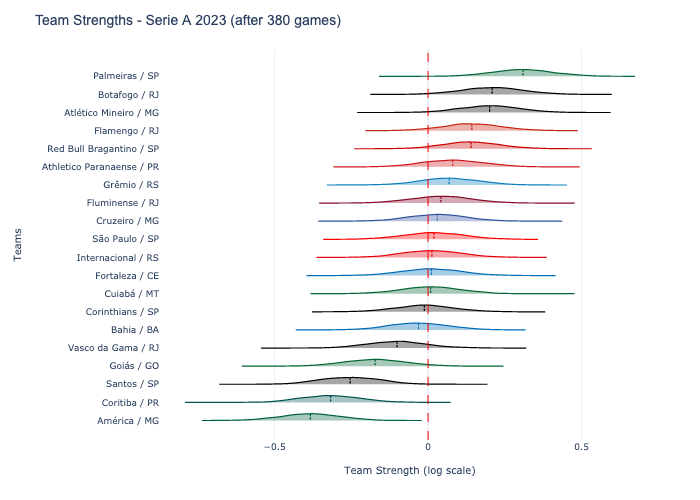
\includegraphics[width=0.9\textwidth]{figures/2023_team_strengths_violin.png}
    \caption{
        \textbf{Posterior distributions of team strengths for the 2023 \textit{Brasileirão} (after 380 matches)}.
        Each violin plot shows the posterior distribution of the team strength parameter (log scale) estimated from 4,000 MCMC samples.
        Teams are ordered vertically by posterior mean strength, from lowest (bottom) to highest (top).
        The shape of each violin represents the density of the posterior distribution, and the dashed line inside each violin indicates the mean.
        The dashed red vertical line at zero represents the average strength.
    }
    \label{fig:team_strengths_2023}
\end{figure}

\subsection{2025 Season}
\label{subsec:season_2025}

If Botafogo collapsed in 2023, in 2024 they had a season with intense competition for the title with Palmeiras.
They won the championship on the last round, after a victory over São Paulo.
The year of Botafogo was also marked by the title of Copa Libertadores, with a 3-1 victory over Atlético Mineiro in the final.
After an eventful year in 2024, we select 2025 as a season with similar title race and because it is more recent.

The 2025 season featured an intense battle between Flamengo and Palmeiras for the title.
In addition to the Brasileirão, Flamengo and Palmeiras also contested the final of Copa Libertadores, with Flamengo winning the title by 1-0.
For Brazilian clubs, these two titles are the most important ones of the season, showing the strength of these clubs.

Figure~\ref{fig:2025_champ} shows the championship probability evolution.
In July, after the FIFA Club World Cup, Flamengo had almost 80\% probability of winning the title.
At this moment, Flamengo had 27 points in 12 games, while Cruzeiro had 24 points in 12 games and Palmeiras 22 points in 11 games.
Until October, Flamengo was leading the championship with similar performance of Palmeiras.
On October 1, Flamengo had 54 points and Palmeiras had 52 points, both with 24 games played.
At this point, both clubs had a similar probability of winning the title.

This equilibrium followed until mid-November, with a jump of Flamengo's probability in mid-October, after a 3-2 victory over Palmeiras, followed by a fall after a loss by 1-0 to Fortaleza.
In November, after a sequence of five consecutive matches without victory, Palmeiras' probability of being champion fell to near zero.
At the penultimate round, Flamengo guaranteed the title by winning their match against Ceará by 1-0.

\begin{figure}[htbp]
    \centering
    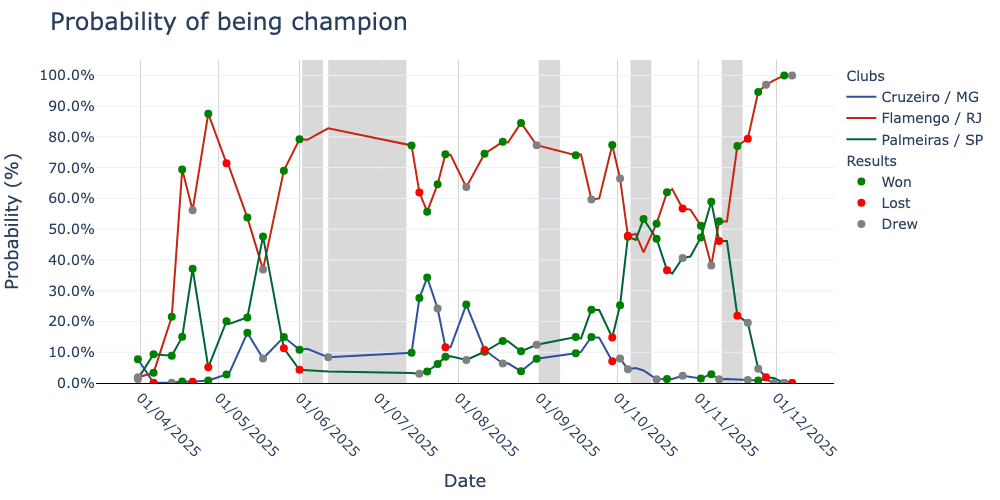
\includegraphics[width=\textwidth]{figures/2025_visualization_poisson_7_champ.png}
    \caption{
        \textbf{Championship probability evolution for the 2025 \textit{Brasileirão}}.
        Each line represents the probability of winning the title for a given club, updated after each match-day.
        Markers indicate individual match results: green circles denote victories, red circles denote defeats, and gray circles denote draws.
        Shaded vertical bands indicate FIFA international break periods.
    }
    \label{fig:2025_champ}
\end{figure}

Like 2023, the relegation battle only finished in the last round.
In this season, the battle was for two positions on the relegation zone, with six clubs with mathematical chances of being relegated: Internacional, Vitória, Fortaleza, Ceará, Santos and Atlético Mineiro.
Atlético's probability was near zero, since they had 3 points more than Vitória, first club in the relegation zone, and a goal difference of -6 goals, while Vitória had a goal difference of -18 goals.
Santos also had a small chance, with a probability of 1.78\%.
Ceará and Fortaleza, both with only one point over the relegation zone, had a probability of 15.71\% and 50.92\%, respectively.
The two clubs that were in the relegation zone, Vitória and Internacional, had a probability of 58.27\% and 73.32\%, respectively.
In the last round, both Vitória and Internacional won their matches, while Fortaleza and Ceará lost, resulting in the relegation of the two rivals.

\begin{figure}[htbp]
    \centering
    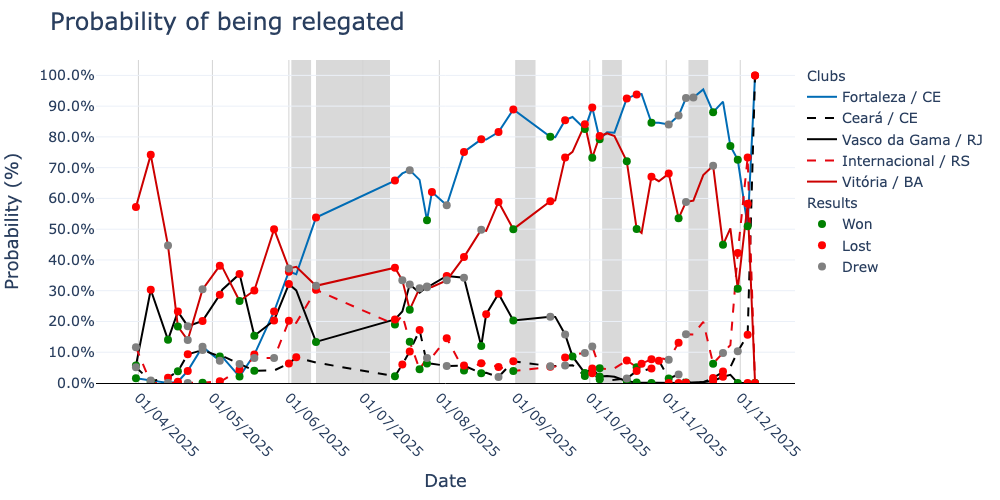
\includegraphics[width=\textwidth]{figures/2025_visualization_poisson_7_z4.png}
    \caption{
        \textbf{Relegation probability evolution for the 2025 \textit{Brasileirão}}.
        Each line represents the probability of relegation (finishing in positions 17--20) for a given club, updated after each match-day.
        Markers indicate individual match results: green circles denote victories, red circles denote defeats, and gray circles denote draws.
        Shaded vertical bands indicate FIFA international break periods.
    }
    \label{fig:2025_z4}
\end{figure}

Figure~\ref{fig:heatmap_2025} shows the mid-season position distribution for all 20 clubs after 189 matches.
Due to the FIFA Club World Cup, some matches were rearranged along the season.
Then at this point, Flamengo had 43 points in 19 games, while Palmeiras had 39 in 18 matches and Cruzeiro had 38 in 20 matches.
Since Flamengo's points are already guaranteed, the probability of Flamengo winning the title, 78.19\%, has a slight bias when compared to Palmeiras, 13.61\%, whose points are yet to be confirmed or Cruzeiro, 6.38\%, which had already played one more game.
Palmeiras and Cruzeiro are the favourites to finish in second and third place, respectively.

A notable feature of 2025 is Mirassol's strong performance.
The club, promoted from \textit{Série B}, shows probability concentrated in positions 4--6, representing one of the best campaigns for a debuting team.
Bahia and Botafogo also occupy positions 4--6, but with a slightly higher probability of finishing in the top four.

At the bottom, Sport shows near-certain relegation probability (95.95\% in positions 17--20).
Juventude, 79.06\%, and Fortaleza, 79.13\%, also exhibit high relegation probabilities.
Vitória shows 49.45\% relegation probability, reflecting their precarious but not hopeless position.
Santos, 25.12\%, Vasco, 22.38\% and Corinthians, 20.36\%, appear in danger but with substantial probability of survival.
At this point, Internacional had only 6.33\% probability of being relegated.

\begin{figure}[htbp]
    \centering
    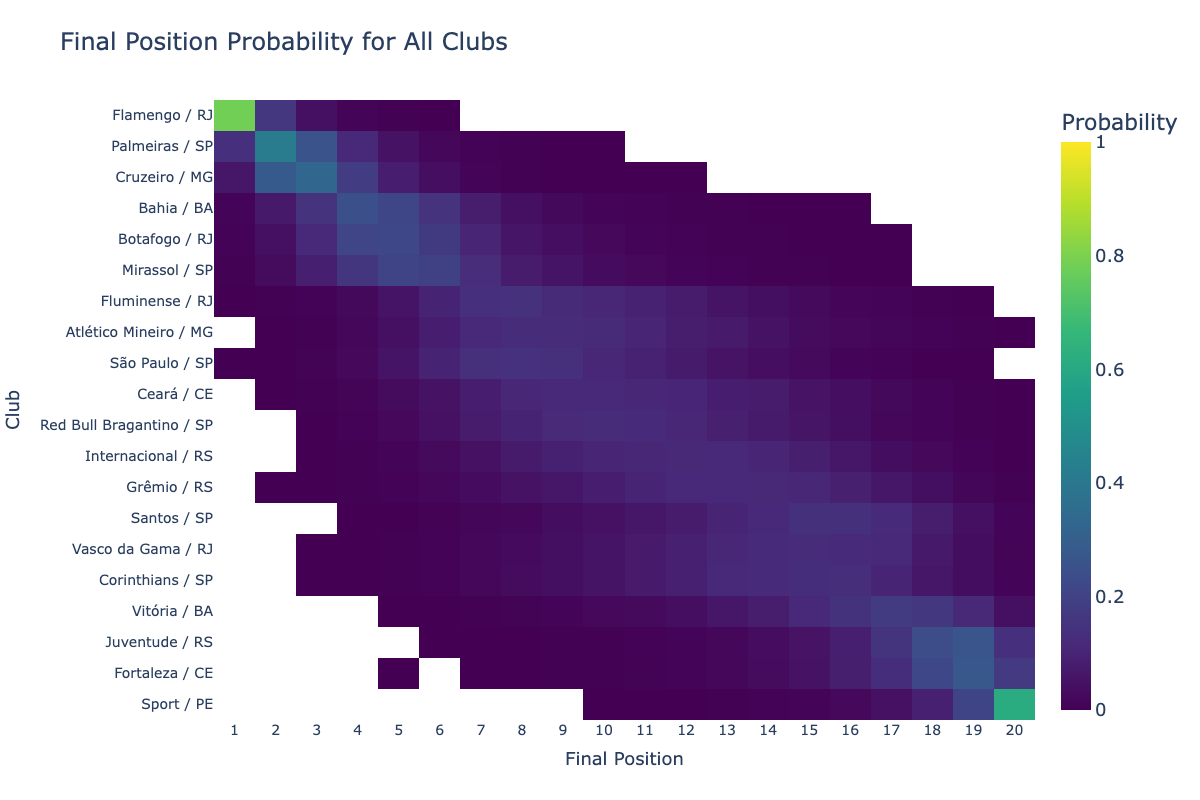
\includegraphics[width=\textwidth]{figures/2025_final_position_probs_all_clubs_189_poisson_7.png}
    \caption{
        \textbf{Final position probability distribution at mid-season 2025 (after 189 matches)}.
        Each cell represents the estimated probability of a club (row) finishing the season in a given position (column), based on 10,000 Monte Carlo simulations of the remaining 191 matches.
        Clubs are ordered vertically by expected final position; brighter colours indicate higher probabilities.
    }
    \label{fig:heatmap_2025}
\end{figure}

The end-of-season team strength estimates are shown in Figure~\ref{fig:team_strengths_2025}.
Flamengo and Palmeiras exhibit the highest estimated strengths, with distributions clearly above the average (zero) and clearly separated from Juventude and Sport.
Flamengo also can be distinguished from Red Bull Bragantino, Internacional, Fortaleza and Vitória.
Cruzeiro, Mirassol and Botafogo form a second group of clubs with similar strengths, all with a considerable overlap with the two top clubs.
Fluminense and Bahia also had a median strength above the average.

In the middle of the table, Atlético Mineiro, Grêmio, São Paulo, Santos, Vasco, Corinthians and Ceará had very similar strength distributions, with a considerable overlap with each other.
Red Bull Bragantino, Internacional, Fortaleza and Vitória also had similar distributions, slightly below the mid-table group.
At the bottom, Juventude and Sport had the lowest median strengths, with a distribution entirely below the average.

\begin{figure}[htbp]
    \centering
    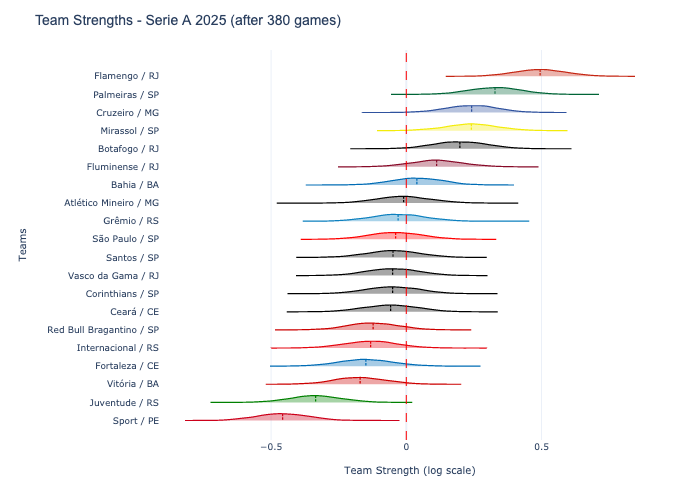
\includegraphics[width=0.9\textwidth]{figures/2025_team_strengths_violin.png}
    \caption{
        \textbf{Posterior distributions of team strengths for the 2025 \textit{Brasileirão} (after 380 matches)}.
        Each violin plot shows the posterior distribution of the team strength parameter (log scale) estimated from 4,000 MCMC samples.
        Teams are ordered vertically by posterior mean strength, from lowest (bottom) to highest (top).
        The shape of each violin represents the density of the posterior distribution, and the dashed line inside each violin indicates the mean.
        The dashed red vertical line at zero represents the average strength.
    }
    \label{fig:team_strengths_2025}
\end{figure}
